\subsection{Results}

\begin{table}[t]
\centering
% centering table
\begin{tabular}{l c c c c c c}
% creating 10 columns
\toprule
% inserting double-line
& \multicolumn{3}{c}{\textsc{Rouge-1}} & \multicolumn{3}{c}{\textsc{Rouge-2}}\\
\cmidrule(lr){2-4}
\cmidrule(lr){5-7}
$\mathrm{Model}$ & $\mathrm{Recall}$ & $\mathrm{Prec.}$ & $\mathrm{F}_1$
& $\mathrm{Recall}$ & $\mathrm{Prec.}$ & $\mathrm{F}_1$\\
\midrule
\textsc{SAP} & $\mathbf{0.282}$ & $\mathbf{0.344}$ & $\mathbf{0.306}$
& $\mathbf{0.045}$ & $\mathbf{0.056}$ & $\mathbf{0.049}$\\
AP          & $0.245$ & $0.285$ & $0.263$ & $0.033$ & $0.038$ & $0.035$ \\
RS          & $0.230$ & $0.271$ & $0.247$  & $0.031$ & $0.037$ & $0.034$ \\
HAC         & $0.169$ & $0.230$ & $0.186$ & $0.017$ & $0.024$ & $0.019$ \\
\bottomrule % inserts single-line
\end{tabular}
%~\\[1ex]
%~\\
%\begin{tabular}{l c c c}
%% creating 10 columns
%\multicolumn{4}{c}{ROUGE-L}\\
%\hline
%\hline
%% inserting double-line
%$\mathrm{System}$ & $\mathrm{Recall}$ & $\mathrm{Prec.}$ & $\mathrm{F}_1$\\[0.5ex]
%\hline
%AP+Salience & $0.275$ & $0.336$ & $0.299$ \\
%AP          & $0.241$ & $0.280$ & $0.258$ \\
%RS          & $0.225$ & $0.265$ & $0.242$ \\
%HAC         & $0.166$ & $0.225$ & $0.182$ \\
%\hline % inserts single-line
%\end{tabular}
%
%
\caption{Model \textsc{Rouge} performance.} % title name of the table
\label{tab:rouge}
%\vspace{-14pt}
\end{table}





\begin{figure}[t]
    \centering
    \begin{tikzpicture}
        \node at (0,0) {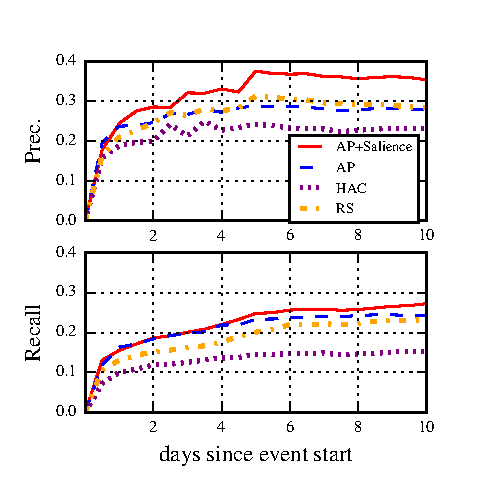
\includegraphics[]{strmsum/figures/rouge-time.eps}};
        \node[draw=white,fill=white,text width=1.05cm] at (2.20,1.55) {};
        \node[draw=white,fill=white,inner sep=0pt,text width=1.05cm] at (2.20,1.60) {\tiny SAP};
        \node[draw=white,fill=white,text width=1.05cm] at (2.20,1.30) {};
        \node[draw=white,fill=white,text width=1.05cm] at (2.20,0.95) {};
        \node[draw=white,fill=white,text width=1.05cm] at (2.20,0.55) {};

        \node[draw=white,fill=white,inner sep=0pt,text width=1.05cm] at (2.20,1.25) {\tiny AP};
        \node[draw=white,fill=white,inner sep=0pt,text width=1.05cm] at (2.20,0.90) {\tiny HAC};
        \node[draw=white,fill=white,inner sep=0pt,text width=1.05cm] at (2.20,0.55) {\tiny RS};
    \end{tikzpicture}
    \caption{System \textsc{Rouge-1} performance over time.}
\label{fig:trouge}
%\vspace{-14pt}
\end{figure}




\paragraph{\textsc{Rouge}} \autoref{tab:rouge} shows our results for system output samples against the 
full summary of nuggets using \textsc{Rouge}. SAP improves over the individual
component systems, i.e. affinity propagation only (AP) or salience prediction
only (RS), suggesting the combination of these two components is beneficial. 
This improvement is statistically 
significant for all ngram precision, recall, and F-measures at the 
$\alpha = .01$ level using the Wilcoxon signed-rank test. 
The full system or the individual components AP and RS also outperform 
the alternative clustering method HAC. 

%Differences between AP and RS
%are relatively small, suggesting they have complentary strengths 



SAP maintains its performance above the baselines over time 
as well. \autoref{fig:trouge} shows the \textsc{Rouge-1} scores over time. We show 
the difference in unigram precision (bigram precision is not shown but it 
follows similar curve). Within the initial days of the event, 
SAP is able to take the lead over the other systems in ngram 
precision. The SAP model is better able to find salient 
updates earlier on; for news and crisis informatics, 
this is an especially important 
quality of the model. 
Moreover, the SAP's recall is not diminished by the high 
precision and remains competitive with \textsc{AP}. Over time 
SAP's recall also begins to pull away, while the other models
begin to plateau.

\begin{figure}[t]
    \centering
\begin{tikzpicture}
  \node at (0,0) {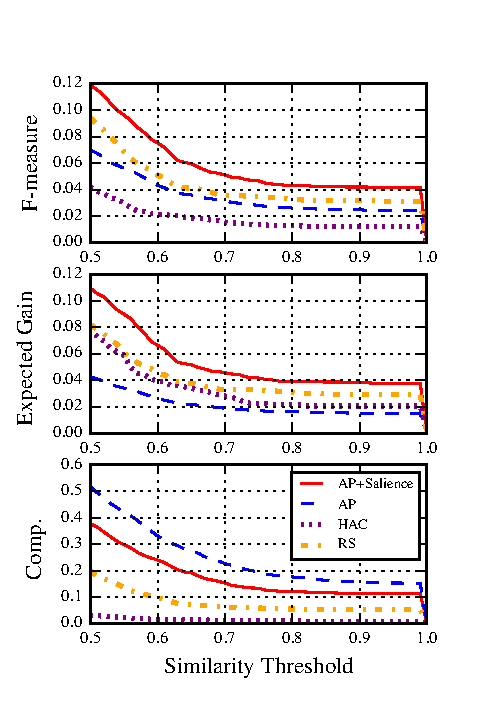
\includegraphics[]{strmsum/figures/nuggets-metrics2.eps}};
    \draw[rectangle,fill=white,draw=white] (2.85,-3.35) rectangle (1.5,-2.1); 
\node[anchor=north west, align=left,font=\tiny,inner sep=0] at (1.5,-2.1) {SAP\\[2.9pt] AP\\[2.9pt] HAC\\[2.9pt] RS};
\end{tikzpicture}
\caption{Expected Gain and Comprehensiveness performance.}
\label{fig:nperf}
%\vspace{-12pt}
\end{figure}




\paragraph{Expected Gain and Comprehensiveness}
\autoref{fig:nperf} shows the expected gain across a range of similarity 
thresholds, where thresholds closer to 1 are more conservative estimates. 
The ranking of the systems remains constant across the sweep with 
\textsc{SAP} beating all baseline systems. Predicting salience in 
general is helpful for keeping a summary on topic as the \textsc{RS} approach 
outperforms the clustering only approaches on expected gain.


When looking at the comprehensiveness of the summaries \textsc{AP} outperforms
\textsc{SAP}. The compromise encoded in the \textsc{SAP} 
objective function, between being representative and being salient, is seen 
clearly here where the performance of the \textsc{SAP} methods is 
lower bounded by the salience focused \textsc{RS} system and upper bounded by 
the clustering only \textsc{AP} system. Overall, \textsc{SAP} achieves
the best balance of these two metrics.


\subsection{Feature Ablation}
\begin{table}[h]
\centering
% centering table
\begin{tabular}{l c c c ccc}
    \toprule
% creating 10 columns
    & \multicolumn{3}{c}{\textsc{Rouge}-1}
    & \multicolumn{3}{c}{\textsc{Rouge}-2}\\
    \cmidrule(lr){2-4} \cmidrule(lr){5-7}
% inserting double-line
$\mathrm{Model}$ & $\mathrm{Recall}$ & $\mathrm{Prec.}$ & $\mathrm{F}_1$
& $\mathrm{Recall}$ & $\mathrm{Prec.}$ & $\mathrm{F}_1$\\
\midrule
Full System & $0.282$ & $0.344$ & $0.306$ & $0.045$ & $0.056$ & $0.049$\\
No Basic    & $0.263$ & $0.380^\dagger$ & $0.294$ & $0.046$ & $0.068^{\dagger\dagger}$ & $0.051^\dagger$\\
No LM       & $0.223^\dagger$ & $0.361$ & $0.254^\dagger$ & $0.033^\dagger$ & $0.056$ & $0.038^\dagger$\\
No Time  & $0.297^\dagger$ & $0.367^{\dagger\dagger}$ & $0.322^\dagger$ & $0.052^{\dagger\dagger}$ & $0.064^{\dagger\dagger}$ & $0.056^{\dagger\dagger}$ \\ 
No Geo   & $0.232^{\dagger\dagger}$ & $0.381$ & $0.265^\dagger$ & $0.037^\dagger$ & $0.065$ & $0.042$ \\  
No Query & $0.251$ & $0.377$ & $0.280$ & $0.043$ & $0.068^\dagger$ & $0.048$ \\
\bottomrule
\end{tabular}
\caption{Feature ablation \textsc{Rouge} performance. 
    $\dagger$ indicates statistically significant difference from 
full model at the $\alpha=.05$ level.
    $\dagger\dagger$ indicates statistically significant difference from 
full model at the $\alpha=.01$ level.
    } % title name of the table
\label{tab:farouge}
\end{table}









\autoref{tab:farouge} shows the results of our feature ablation tests. 
Removing the language models yields a statistically significant drop in both 
ngram recall and F-measure. 

Removing the language model and geographic relevance features leads to a
statistically significant drop in \textsc{Rouge-1} F1 scores. Unfortunately,
this is not the case for the temporal relevance features. We surmise that
these features are too strongly correlated with each other, 
i.e. the differences in TF-IDF between hours are definitely not i.i.d. 
variables. 

Interestingly, removing the basic features leads 
to an increase in both unigram and bigram precision; in the bigram case this 
is enough to cause a statistically significant increase in F-measure over the 
full model. In other words, the generic features actually lead to an inferior 
model when we can incorporate more appropriate domain specific features.
This result perhaps echoes the claim of \cite{ksj98} that generic approaches to 
summarization are unlikely to produce truly useful summaries.





